%!TEX root = stoh_modeling.tex
\section{Модель}
\begin{figure}[h]
  \center{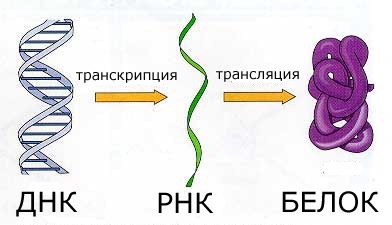
\includegraphics[width=1\linewidth]{dogma-dna-rna-protein}}
\end{figure}
\subsection{Реакции присоединения/отсоединения ТФ}
\begin{figure}[!h]
  \center{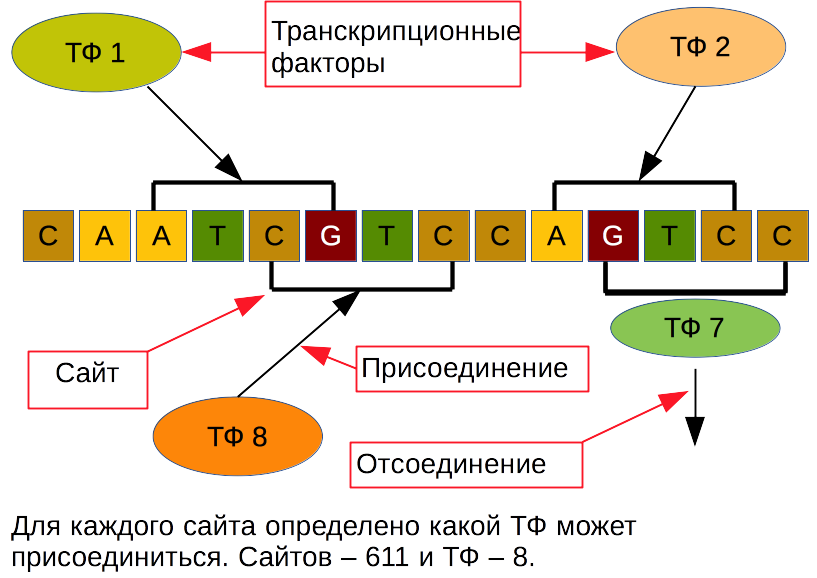
\includegraphics[width=1\linewidth]{geene_exp1}}
\end{figure}
\subsection{Реакции транскрипции и трансляции}
\begin{figure}[!h]
  \center{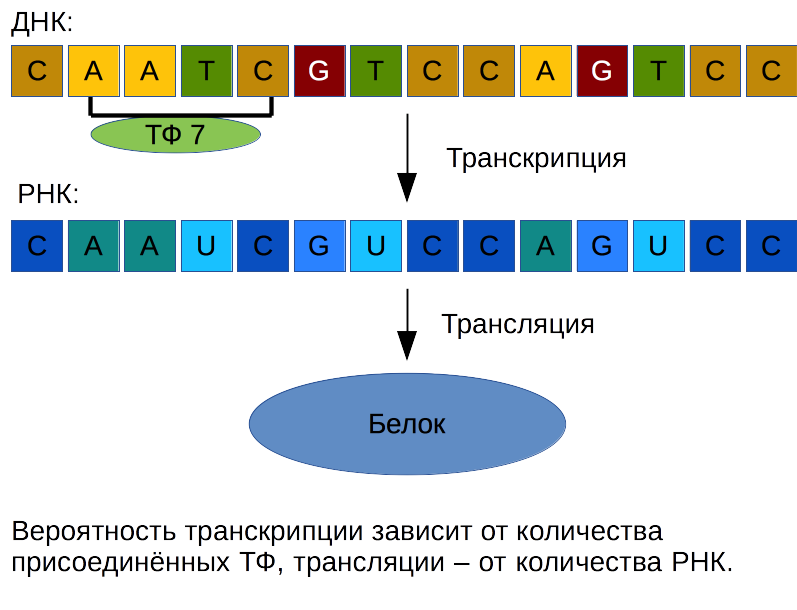
\includegraphics[width=1\linewidth]{geene_exp2}}
\end{figure}
\subsection{Реакции диффузии и деградации}
\begin{figure}[!h]
  \center{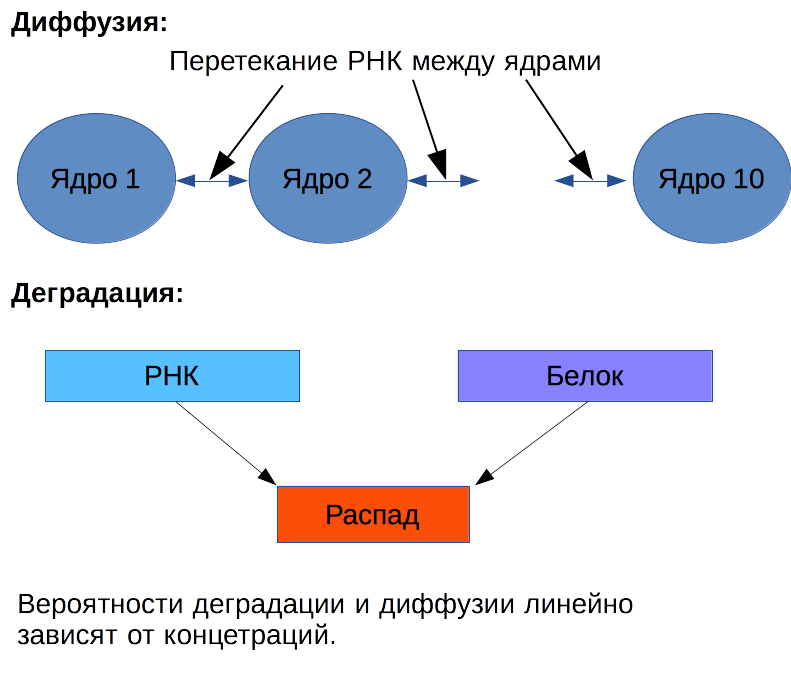
\includegraphics[width=1\linewidth]{geene_exp3}}
\end{figure}
